\section{Arbol de Problemas}

\begin{figure}[H]
    \centering
    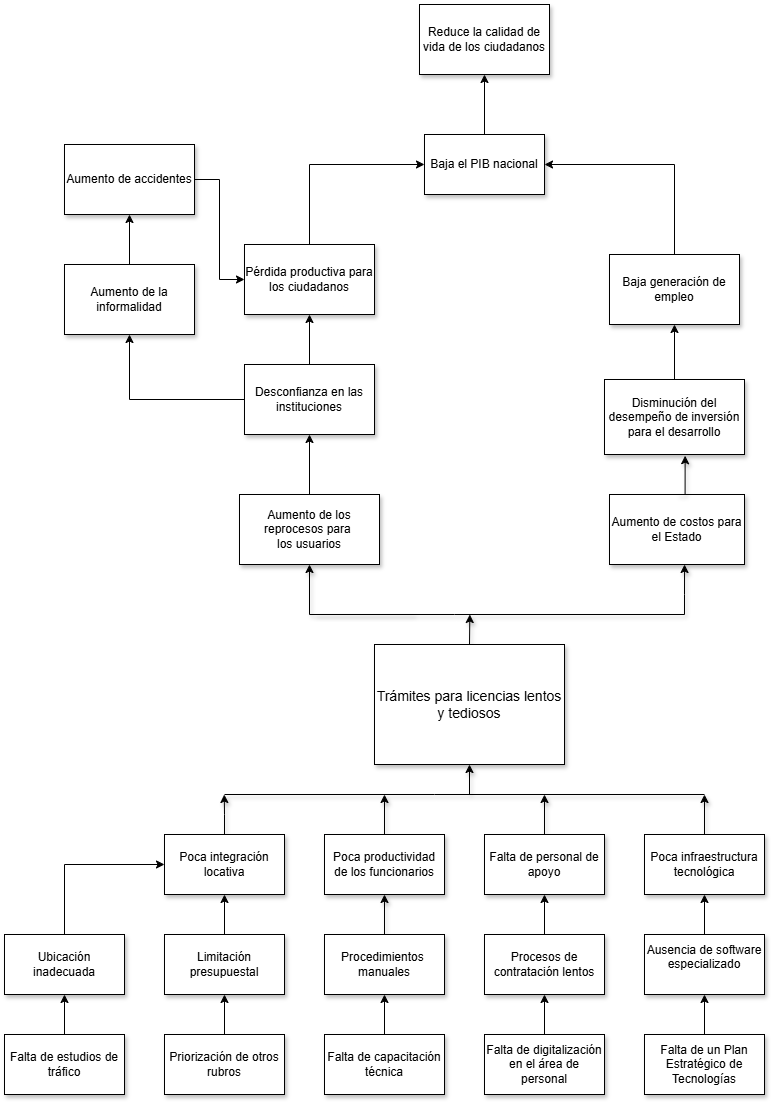
\includegraphics[width=0.9\linewidth]{formulacion/problems-tree/img/arbol_problemas.png}
    \caption{Arbol de Problemas.}
    \label{fig:placeholder}
    \vspace{0.2cm}
    \small Fuente: Elaboración propia.
\end{figure}

\subsection{Fundamentos del Árbol de Problemas}
\begin{itemize}
\item \textbf{Poca integración locativa} \\
En Colombia, la falta de articulación entre los organismos de tránsito municipales y departamentales y la infraestructura urbana ha generado congestión y sobrecarga en los puntos de atención. El crecimiento sostenido del parque automotor en el país ha superado la capacidad física de muchas sedes de tránsito, especialmente en ciudades intermedias, lo que provoca saturación en la atención presencial y congestión vial en zonas cercanas a estas oficinas.  
\textbf{(Ministerio de Transporte, 2024; DANE, 2024)}

\item \textbf{Ubicación inadecuada} \\
Múltiples sedes de tránsito se encuentran en zonas de difícil acceso o con alta congestión vehicular previa, sin estudios técnicos de movilidad que respalden su localización. Esto dificulta la llegada de usuarios y agrava el tráfico circundante, generando barreras físicas para la realización de trámites.  
\textbf{(Ministerio de Transporte, 2024; Asuntos Legales, 2023)}

\item \textbf{Falta de estudios de tráfico} \\
La ausencia de análisis previos sobre flujos vehiculares y peatonales al establecer puntos de atención resulta en colapsos operativos. Sin estos estudios, no se prevén bahías de parqueo ni accesos suficientes, improvisando soluciones sobre la marcha.  
\textbf{(Ministerio de Transporte, 2018; DANE, 2024)}

\item \textbf{Limitación presupuestal} \\
Las restricciones financieras de los gobiernos locales impiden la modernización y ampliación de sedes. Muchos organismos dependen de recursos propios limitados que se destinan prioritariamente a funcionamiento básico, dejando sin inversión la mejora locativa.  
\textbf{(Contraloría General de la República, 2023; Función Pública, 2023)}

\item \textbf{Priorización de otros rubros} \\
En los presupuestos municipales, sectores como salud o educación suelen tener prelación sobre la infraestructura de tránsito. Esto relega las inversiones necesarias para descongestionar y adecuar las oficinas de atención al ciudadano.  
\textbf{(Consejo Privado de Competitividad, 2024; Contraloría General de la República, 2023)}

\item \textbf{Poca productividad de los funcionarios} \\
A nivel nacional, los trámites para obtener o renovar licencias pueden tardar varias semanas dependiendo del municipio. Aunque existe el sistema centralizado del RUNT, muchos procesos requieren validaciones manuales y múltiples pasos presenciales, reduciendo la eficiencia operativa.  
\textbf{(RUNT, 2024; Función Pública, 2023)}

\item \textbf{Procedimientos manuales} \\
En múltiples regiones de Colombia aún se exige la entrega física de documentos, validaciones presenciales y revisión manual de requisitos. Estos procedimientos ralentizan la atención, incrementan el margen de error humano y generan reprocesos innecesarios.  
\textbf{(Función Pública, 2023; Consejo Privado de Competitividad, 2024)}

\item \textbf{Falta de capacitación técnica} \\
Los funcionarios frecuentemente carecen de formación actualizada en nuevas normativas y herramientas digitales, lo que genera errores en la operación del RUNT y demoras en la atención al usuario por desconocimiento de procedimientos.  
\textbf{(Función Pública, 2023; RUNT, 2024)}

\item \textbf{Falta de personal de apoyo} \\
En diversas regiones del país, los organismos de tránsito presentan déficit de agentes y personal administrativo, lo que limita la capacidad para atender trámites. El crecimiento del parque automotor no ha sido proporcional al aumento del talento humano, generando sobrecarga laboral.  
\textbf{(Ministerio de Transporte, 2024; Contraloría General de la República, 2023)}

\item \textbf{Procesos de contratación lentos} \\
La burocracia en la vinculación de nuevo personal impide cubrir vacantes con agilidad, especialmente en temporadas de alta demanda. Los trámites administrativos para autorizar contrataciones pueden tomar meses, dejando las sedes suboperativas.  
\textbf{(Función Pública, 2023; Contraloría General de la República, 2023)}

\item \textbf{Falta de digitalización en el área de personal} \\
La gestión del talento humano en estas entidades suele ser manual, sin sistemas que agilicen la selección y asignación de turnos. Esto dificulta responder dinámicamente a las necesidades operativas del servicio.  
\textbf{(Función Pública, 2023; Ministerio TIC, 2024)}

\item \textbf{Poca infraestructura tecnológica} \\
Aunque el Gobierno Nacional ha promovido la digitalización, muchas oficinas presentan sistemas con baja interoperabilidad y dependencia de servidores centrales. Las fallas en plataformas digitales afectan la continuidad de los trámites en diferentes regiones.  
\textbf{(RUNT, 2024; Ministerio TIC, 2024)}

\item \textbf{Ausencia de software especializado} \\
Muchas sedes operan con herramientas ofimáticas básicas en lugar de software de gestión de tránsito integrado. Esto fragmenta la información y obliga a recapturas de datos que deberían ser automáticas.  
\textbf{(Ministerio TIC, 2024; Procuraduría General, 2024)}

\item \textbf{Falta de un Plan Estratégico de Tecnologías} \\
La carencia de una hoja de ruta tecnológica a largo plazo lleva a inversiones desarticuladas y obsolescencia rápida de equipos. Sin un plan PETI claro, las adquisiciones no resuelven los problemas estructurales de conectividad y procesamiento.  
\textbf{(Ministerio TIC, 2024; Consejo Privado de Competitividad, 2024)}

\item \textbf{Problemática principal: Trámites para licencias lentos y tediosos} \\
En Colombia, la gestión de licencias presenta demoras constantes y procesos extensos. En distintas ciudades se reportan largas filas para renovar o expedir la licencia, evidenciando una alta dependencia tecnológica y limitada capacidad operativa ante fallas del RUNT.  
\textbf{(RUNT, 2024; Ministerio de Transporte, 2024)}

\item \textbf{Aumento de los reprocesos para los usuarios} \\
Las fallas en el RUNT y la baja interoperabilidad generan reprocesos frecuentes. Los usuarios deben reagendar citas o repetir documentos, aumentando costos económicos y emocionales.  
\textbf{(RUNT, 2024; Función Pública, 2023)}

\item \textbf{Desconfianza en las instituciones} \\
La ineficiencia percibida y los constantes fallos del sistema erosionan la credibilidad de los organismos de tránsito. Los ciudadanos perciben la gestión como negligente, lo que dificulta la implementación de nuevas políticas públicas.  
\textbf{(Consejo Privado de Competitividad, 2024; Función Pública, 2023)}

\item \textbf{Aumento de la informalidad} \\
Ante las barreras para obtener documentos legales, crece el mercado de tramitadores ilegales y la falsificación de licencias. Esto crea un subregistro de conductores no aptos circulando en las vías.  
\textbf{(Ministerio de Transporte, 2024; Fiscalía General de la Nación, 2024)}

\item \textbf{Aumento de accidentes} \\
La circulación de conductores sin licencia o con documentos obtenidos irregularmente incrementa la siniestralidad vial, ya que no han validado sus competencias teóricas y prácticas idóneamente.  
\textbf{(Agencia Nacional de Seguridad Vial, 2024; Ministerio de Transporte, 2024)}

\item \textbf{Pérdida productiva para los ciudadanos} \\
El tiempo invertido en trámites reduce la productividad laboral. Las empresas destinan miles de horas a procesos burocráticos, impactando a trabajadores independientes que dependen del vehículo.  
\textbf{(Consejo Privado de Competitividad, 2024; DANE, 2024)}

\item \textbf{Baja del PIB nacional} \\
La acumulación de ineficiencias impacta la competitividad del país. Los retrasos en trámites de movilidad afectan sectores estratégicos como logística e infraestructura, reduciendo el impulso productivo.  
\textbf{(Consejo Privado de Competitividad, 2024; DANE, 2024)}

\item \textbf{Reduce la calidad de vida de los ciudadanos} \\
El estrés generado por los trámites, sumado a las pérdidas económicas y de tiempo, deteriora el bienestar general de la población, afectando su satisfacción con el entorno urbano y los servicios del Estado.  
\textbf{(DANE, 2024; Departamento Nacional de Planeación, 2023)}

\item \textbf{Aumento de costos para el Estado} \\
La ineficiencia incrementa el gasto público al mantener sistemas desactualizados y requerir más personal operativo para subsanar fallas manuales, desviando recursos de inversión.  
\textbf{(Contraloría General de la República, 2023; Función Pública, 2023)}

\item \textbf{Disminución del desempeño de inversión para el desarrollo} \\
Los recursos atrapados en gastos de funcionamiento ineficiente dejan de invertirse en proyectos de desarrollo vial y tecnológico, frenando la modernización del sector transporte.  
\textbf{(Consejo Privado de Competitividad, 2024; Ministerio de Transporte, 2024)}

\item \textbf{Baja generación de empleo} \\
La falta de dinamismo en el sector transporte y las trabas para legalizar conductores profesionales limitan la creación de nuevos puestos de trabajo formales en empresas de logística y movilidad.  
\textbf{(DANE, 2024; Gremios del Transporte, 2024)}

\end{itemize}